\section{Pravidlo součinu a součtu}

Vezměme si pro začátek jednu motivační úlohu.

\begin{exercise}
    \textit{Předpokládejme, že chceme zjistit počet různých kurzů nabízených Wisconsinskou univerzitou v Madisonu. Kurzy rozdělíme podle oddělení, na kterém jsou uvedeny. Za předpokladu, že nedochází ke křížovému vypisování (křížové vypisování nastává, když je stejný kurz vypsán na více než jedné katedře), kolik předmětů si můžeme jako studenti zapsat?} \citep[str. 28]{Brualdi2018}
\end{exercise}

\begin{solution}\label{exercise:addition_principle}
    K problému můžeme přistoupit následovně: předměty si postupně rozdělíme do množin. Množinu všech dostupných předmětů si označíme $C$ (z angl. \emph{classes}). To znamená, že hledáme $\sizeof{C}$. Předměty si rozdělíme do množin podle katedry, která je nabízí. Tedy máme-li na univerzitě, pro zjednodušení, např. 5 kateder, pak se nám předměty rozdělí do pěti množin, které si označíme $C_1,\,\dots,\, C_5$. Množina všech předmětů $C$ je jednoduše sjednocením předmětů z jednotlivých kateder $C_1,\,\dots,\, C_5$, tj.
    \begin{equation*}
        C=\bigcup\limits_{i=1}^{5}C_i=C_1\cup C_2\cup C_3\cup C_4\cup C_5\,.
    \end{equation*}
    Protože ze zadání víme, že každý předmět je vypsán v rámci \textbf{právě jedné} katedry, pak množiny $C_1,\,\dots,\, C_5$ jsou po dvou disjunktní. Takže nám jednoduše stačí spočítat předměty na jednotlivých katedrách
    \begin{equation*}
        \sizeof{C}=\sum_{i=1}^{5}\sizeof{C_i}=\sizeof{C_1}+\sizeof{C_2}+\sizeof{C_3}+\sizeof{C_4}+\sizeof{C_5}\,.
    \end{equation*}
\end{solution}

Ačkoliv jsme úlohu \ref{exercise:addition_principle} jsme řešili sice trochu složitě, intuitivně je tento způsob nejspíše jasný. Máme-li $n_1$ způsobů, jak provést určitou akci a $n_2$ způsobů, jak provést nějakou jinou akci (kterou nelze provést současně s první), pak máme dohromady $n_1+n_2$ způsobů, jak vybrat některou činnost.\par
Z tohoto jednoduchého principu plyne tzv. \emph{kombinatorické pravidlo součtu}, které budeme v dalších úlohách využívat.

\begin{theorem}[Kombinatorické pravidlo součtu]\label{thm:pravidlo_souctu}
    Jsou-li $X_1,\,X_2,\,\dots,\,X_n$ konečné množiny, které jsou po dvou disjunktní, pak platí
    \begin{equation*}
        \sizeof{X_1\cup X_2\cup\dots\cup X_n}=\sizeof{X_1}+\sizeof{X_2}+\dots+\sizeof{X_n}
    \end{equation*}
    nebo zkráceně
    \begin{equation*}
        \sizeof{\bigcup\limits_{i=1}^{n}X_i}=\sum_{i=1}^{n}\sizeof{X_i}.
    \end{equation*}
\end{theorem}

Představme si, že máme městečka $A,\,B,\,C$, mezi nimiž vede po řadě 3 a 5 cest (tj. 3 cesty mezi $A$ a $B$, 4 cesty mezi $B$ a $C$).

\begin{figure}[H]
	\centering
	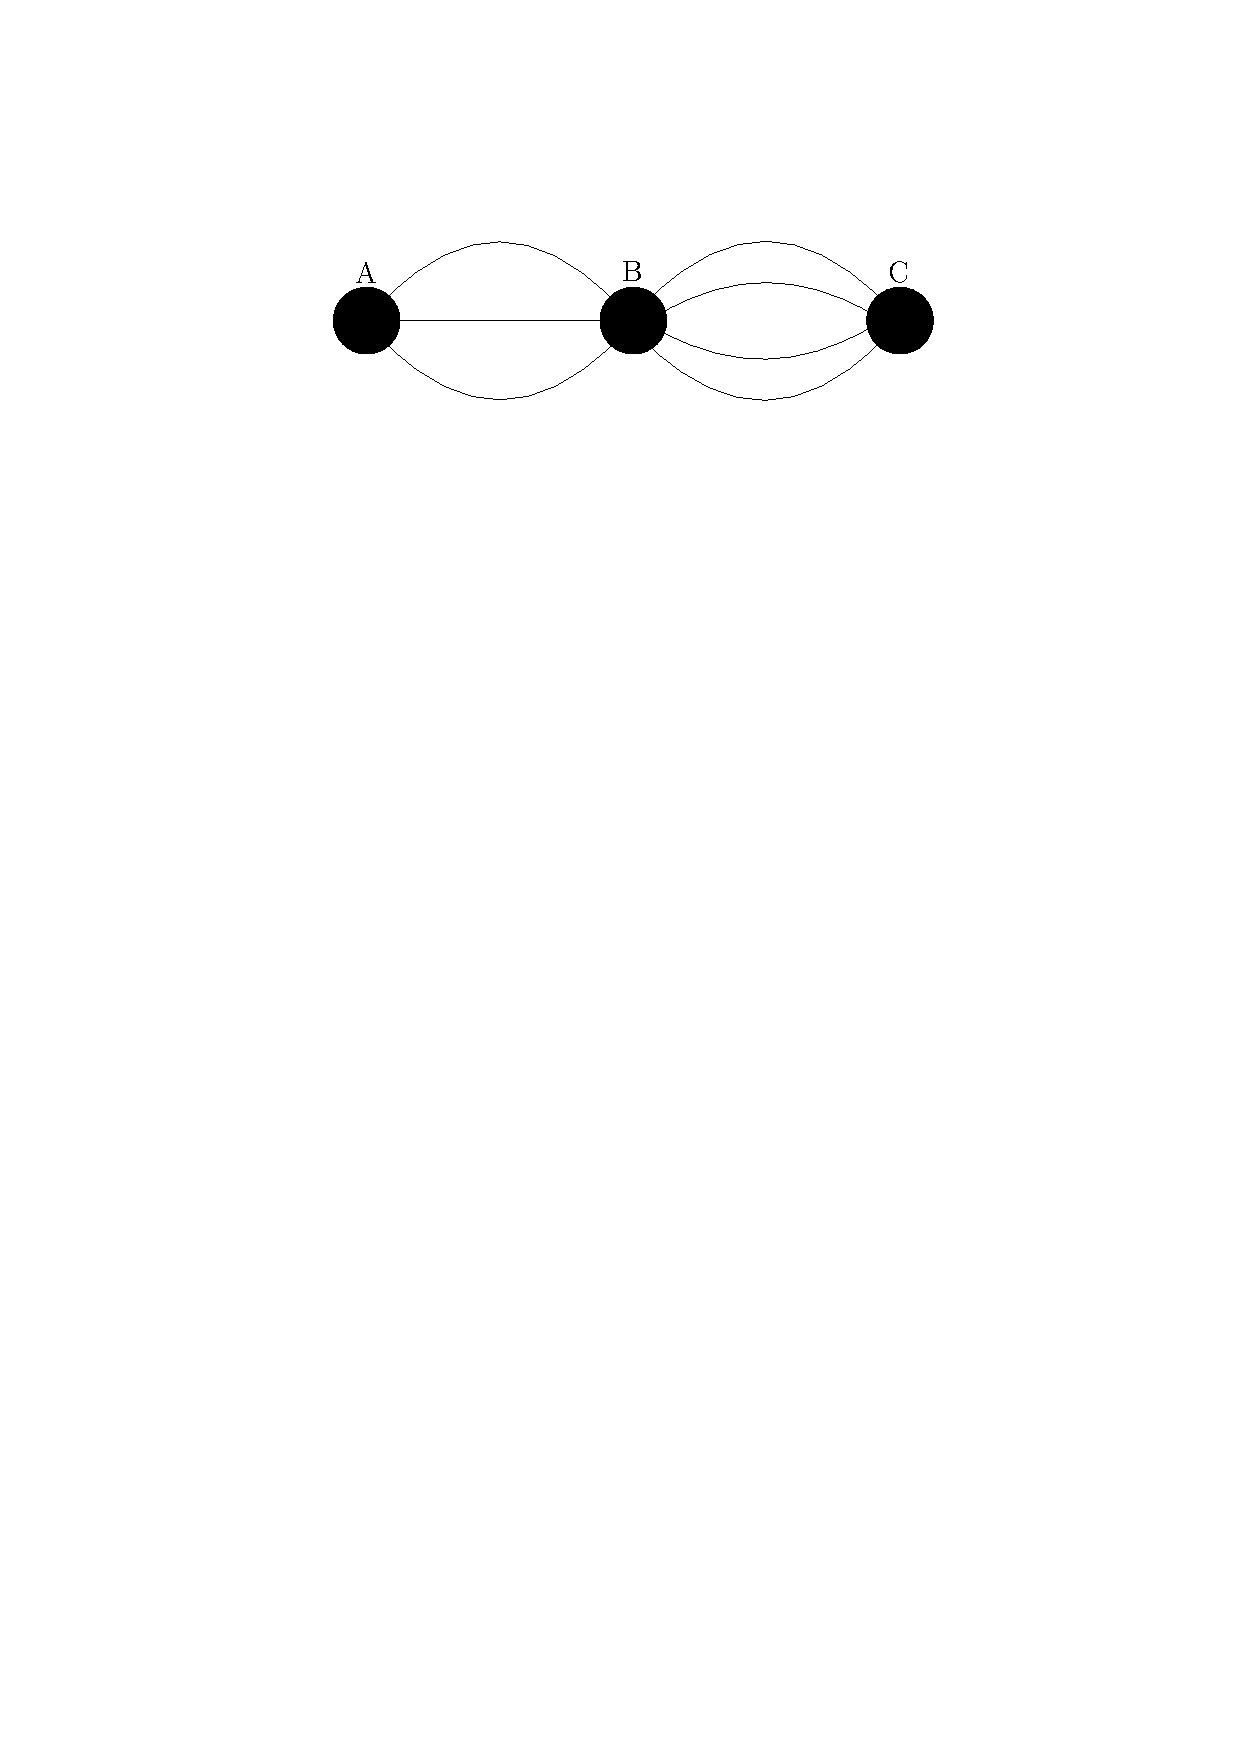
\includegraphics[scale=\normalipe]{ch02_mesta.pdf}
    \caption{Cesty mezi městy $A,\,B,\,C$.}
    \label{fig:mesta}
\end{figure}

Chceme zjistit počet všech způsobů, jak se dostat z města $A$ do města $C$. Jak aplikujeme pravidlo součtu zde? Mohli bychom si zde rozdělit cesty z $A$ do $C$ do množin podle toho, kterou cestou jsme dorazili z $A$ do $B$. Pokud tak učiníme, pak jsme rozdělili cesty do celkem tří množin $P_1,\,P_2,\,P_3$, přičemž všechny jsou po dvou disjunktní (žádná z cest z $A$ do $C$ nemůže obsahovat dvě různé cesty z $A$ do $B$) a množina $P$ obsahuje všechny cesty z $A$ do $C$. Tedy celkový počet cest $\sizeof{P}$ je roven součtu $\sizeof{P_1}+\sizeof{P_2}+\sizeof{P_3}$. Pro každou cestu mezi městy $A$ a $B$ máme 4 možnosti, kudy se dostat z $B$ do $C$. Tedy
\begin{equation*}
    \sizeof{P_1}=\sizeof{P_2}=\sizeof{P_3}=4.
\end{equation*}
To znamená, že celkový počet cest $\sizeof{P}=\sizeof{P_1}+\sizeof{P_2}+\sizeof{P_3}=4+4+4=3\cdot 4=12.$.\par
Tento způsob je jistě velmi nepraktický a navíc je celkem očividné, že na daný výsledek jsme mohli přijít hned. Stačilo vynásobit počet cest mezi městy $A$ a $B$ a počet cest mezi městy $B$ a $C$. Z toho dostáváme druhé kombinatorické pravidlo:

\begin{theorem}[Kombinatorické pravidlo součinu]\label{thm:pravidlo_soucinu}
    Počet uspořádaných $k$-tic, jejichž $i$-tý člen lze vybrat $n_i$ způsoby je roven
    \begin{equation*}
        n_1\cdot n_2\cdot\dots\cdot n_k = \prod_{i=1}^{k}n_i
    \end{equation*}
\end{theorem}
Je důležité zmínit, že jednotlivé výběry \textbf{musí být nezávislé}, tedy výběr na jednu pozici nesmí ovlivnit počet výběrů na ostatní pozice. Méně formálně, avšak užitečněji, můžeme pravidlo formulovat i takto: \textit{Lze-li první výběr provést celkem $n$ způsoby a druhý výběr $m$ způsoby bez ohledu na první výběr, pak celkový počet dvojic možných výběrů je $nm$.} (Pochopitelně, toto lze zobecnit na libovolný počet výběrů, jako je tomu v \ref{thm:pravidlo_soucinu}.)

\begin{exercise}
    Křídy jsou vyráběny
    \begin{itemize}
        \item ve 3 různých barvách,
        \item v 8 různých délkách
        \item a o 4 různých průměrech.
    \end{itemize}
    Kolik typů kříd celkově lze zakoupit? \citep[str. 29]{Brualdi2018}
\end{exercise}
\begin{solution}
    Barvu křídy můžeme vybrat celkem třemi způsoby, délku osmi způsoby a průměr křídy celkem čtyřmi způsoby. Protože výběry jsou na sobě nezávislé, pak podle předchozího pravidla součinu existuje celkem $3\cdot 8\cdot 4=96$ typů kříd.
\end{solution}

\begin{exercise}
    Kolik čtyřciferných přirozených čísel lze sestavit z cifer 0, 1, 2, 3, 4, 5, jestliže
    \begin{enumerate}[label=(\alph*)]
        \item cifry se mohou opakovat,
        \item cifry se nemohou opakovat?
    \end{enumerate}
    (Úloha i řešení \citep[str. 7]{Slavik2022}.)
\end{exercise}
\begin{solution}{Řešení (a)}
    Protože se cifry mohou opakovat, pak na každé číselné pozici máme stejný počet možností výběru číslici, až na první pozici, neboť nemůžeme vybrat číslici 0 (jinak by se nejednalo o \emph{čtyřciferné} číslo). Na první pozici máme tak 5 možností výběru a na zbylých třech máme 6 možností, tj. celkově existuje
    \begin{equation*}
        5\cdot 6\cdot 6\cdot 6 = 1080\;\text{možností.}
    \end{equation*}
\end{solution}
\begin{solution}{Řešení (b)}
    Tentokrát se cifry nesmí opakovat. Úvaha tak zůstává stejná, ale při určování počtu možností výběru musíme zohlednit již vybrané číslice. Na první pozici tak máme 5 možností výběru (nesmíme vybrat nulu), na druhé pozici máme 5 možností (původně jsme měli 6, ale jednu cifru jsme již použili na první pozici), na třetí pozici máme 4 možnosti (2 číslice jsme již použili) a na čtvrté pozici máme 3 možnosti. Celkově tak existuje
    \begin{equation*}
        5\cdot 5\cdot 4\cdot 3=300\;\text{možností.}
    \end{equation*}
\end{solution}

Kombinatorické pravidlo součtu a součinu však můžeme v různých úlohách kombinovat. Speciálně, pokud si tak ulehčíme hledání určených konfigurací.

\begin{exercise}
    Kolik sudých čísel čtyřciferných přirozených čísel lze sestavit z cifer 0, 1, 2, 3, 4, 5, jestliže se nesmí opakovat? (Úloha i řešení \citep[str. 8]{Slavik2022}.)
\end{exercise}
\begin{solution}
    Aby výsledné číslo bylo sudé, musí končit (tj. mít na čtvrté pozici) číslici 0, 2, nebo 4. Zde již však nastává problém, neboť nemůžeme hned aplikovat pravidlo součinu. Je tomu tak proto, že pokud by byla na čtvrté pozici nula, pak na první pozici máme 5 možností, zatímco pokud by zde byla číslice 2, nebo 4, pak počet přípustných číslic na první pozici je již pouze 4 (nesmíme vybrat číslici 0 a pak číslici na čtvrté pozici). Počet výběrů tak již není nezávislý. Nicméně můžeme každý z případů vyšetřit zvlášť:
    \begin{itemize}
        \item označme si množinu $D_1$ (z angl. \emph{digit}) obsahující všechna čísla končící číslicí 0,
        \item množinu čísel $D_2$ končících číslicí 2 a
        \item množinu čísel $D_3$ končících číslicí 4.
    \end{itemize}
    Pro čísla končící nulou máme na první pozici celkem 5 možností, na druhé pak 4 možnosti a na třetí 3 možnosti. Tedy z kombinatorického pravidla součinu máme
    \begin{equation*}
        \sizeof{D_1}=5\cdot 4\cdot 3=60\;\text{možností.}
    \end{equation*}
    Množiny $D_2$ a $D_3$ mají stejnou velikost, neboť v obou případech máme na první pozici 4 možnosti výběru, na druhé 4 možnosti výběru a na třetí 3 možnosti. Tj.
    \begin{equation*}
        \sizeof{D_2}=\sizeof{D_3}=4\cdot 4\cdot 3=48\;\text{možností.}
    \end{equation*}
    Je jasné, že tyto množiny jsou disjunktní (každá dvojice množin obsahuje čísla s jinou číslicí na čtvrté pozici). Tedy podle kombinatorického principu součtu platí
    \begin{equation*}
        \sizeof{D_1\cup D_2\cup D_3}=\sizeof{D_1}+\sizeof{D_2}+\sizeof{D_3}=60+48+48=156\;\text{možností.}
    \end{equation*}
\end{solution}